\documentclass{nime-alternate} 
\usepackage{anonymize}
\usepackage{hyperref}
\usepackage[utf8]{inputenc}
\title{Enhancing Violin Performance through Real-Time Interaction: Design and Evaluation of a Wireless Audio-Visual Interface}
% \conferenceinfo{NIME'23,}{31 May–2 June, 2023, Mexico City, Mexico.}
\label{key}
\numberofauthors{3}
\author{
\alignauthor
Anon Anonymous\\
       \affaddr{\anonymize{Institute for Anonymous}}\\
       \affaddr{\anonymize{1932 Wallamaloo Lane}}\\
       \affaddr{\anonymize{Wallamaloo, New Zealand}}\\
       \email{\anonymize{trovato@corporation.com}}
\alignauthor
Anon Anonymous\\
       \affaddr{\anonymize{Institute for Anonymous}}\\
       \affaddr{\anonymize{1932 Wallamaloo Lane}}\\
       \affaddr{\anonymize{Wallamaloo, New Zealand}}\\
       \email{\anonymize{trovato@corporation.com}}
\alignauthor
Anon Anonymous\\
       \affaddr{\anonymize{Institute for Anonymous}}\\
       \affaddr{\anonymize{1932 Wallamaloo Lane}}\\
       \affaddr{\anonymize{Wallamaloo, New Zealand}}\\
       \email{\anonymize{trovato@corporation.com}}
}


\begin{document}

\maketitle

\begin{abstract}

This paper presents a detailed description of the development of a wireless audio-visual interface that is integrated with a violin bow. 
This interface is a work-in-progress prototype resulting from a practice-based research project into optimal physical design and software mappings for the virtuoso string player.
As an augmented instrument, this interface aims at extending the existing skill set of the performer. Moving away from gestural analysis approaches, we focus more directly on optimising real-time performer interaction and control for violin performance, using bow hand fingers to manipulate the interface. A further novel aspect is the equal emphasis placed on both the audio and visual real-time processing which unlocks potential for new compositional possibilities and interdisciplinary performance situations.
The interface is intentionally minimally invasive and wireless so as to reduce performer movement restrictions as well as permanent modifications to the violin bow. We contextualize our research process and outcomes within two performance situations, basing future design possibilities on the evaluation of an expert violinist.



\end{abstract} 




\keywords{Augmented Instruments, physical prototyping, interface design, violin, audio-visual}
\ccsdesc[500]{Human-centered computing~Interface design prototyping}
\ccsdesc[100]{Applied computing~Performing arts}
\ccsdesc[300]{Applied computing~Sound and music computing}

% this line creates the CCS Concepts section.
\printccsdesc

% \textbf{Please read the comments starting on line 140 of the nime-template.tex file to see how to create the CCS Concept Classifications!} % Remove this line in your paper!

\section{Introduction}

% What is the problem???
% - lots of augmented string instruments extending normal performance gestures.
% - some interfaces add new performance gestures as well as extending existing possibilities.
% - most are integrated directly into the instrument and cannot be removed, and or are not visually discrete.
% - how to approach audio-visual composition?
% - degrees of freedom

Acoustic bowed string instruments have been enhanced with a variety of technologies as a means of gestural analysis and new expressive possibilities by many researchers\cite{overholt:advancements} \cite{young:hyperbow} \cite{bevilacqua:augmented} \cite{machover:hyperinstrument} \cite{rose:interactive} \cite{kimura:extracting}. Primarily, these technologies have consisted of various sensors analysing the string player's physical idiosyncrasies as well as the inherent physics of the instrument itself\cite{overholt:musical}\cite{miranda:new}. The chosen sensors are integrated with the body or the bow of the instrument and in some cases, the performing artist\cite{reid:women}\cite{van:musicjacket}. The collected sensor data is mapped within an appropriate musical software environment aiming to create a novel, meaningful and expressive creative output. Although multiple and varied approaches to augmenting the acoustic violin have been developed, our prototype strives to explore the space between real-time normal player gestural analysis and new digital instrument design, emphasising interactivity and minimal invasion.

In this paper we discuss the development of a new wireless audio-visual interface with design considerations that focus on optimal sensor placement for real-time performer right hand manipulation and gestural analysis.
We discuss our approaches to sensor choices as well as detailing our software design parameters which place equal importance on both audio and visual software mappings. We present our work-in-progress interface within the context of two distinctly varied performances, reflecting on each situation from the first author's researcher/practitioner perspective and concluding with future creative design and output directions.

\begin{figure}[t]
	\centering
		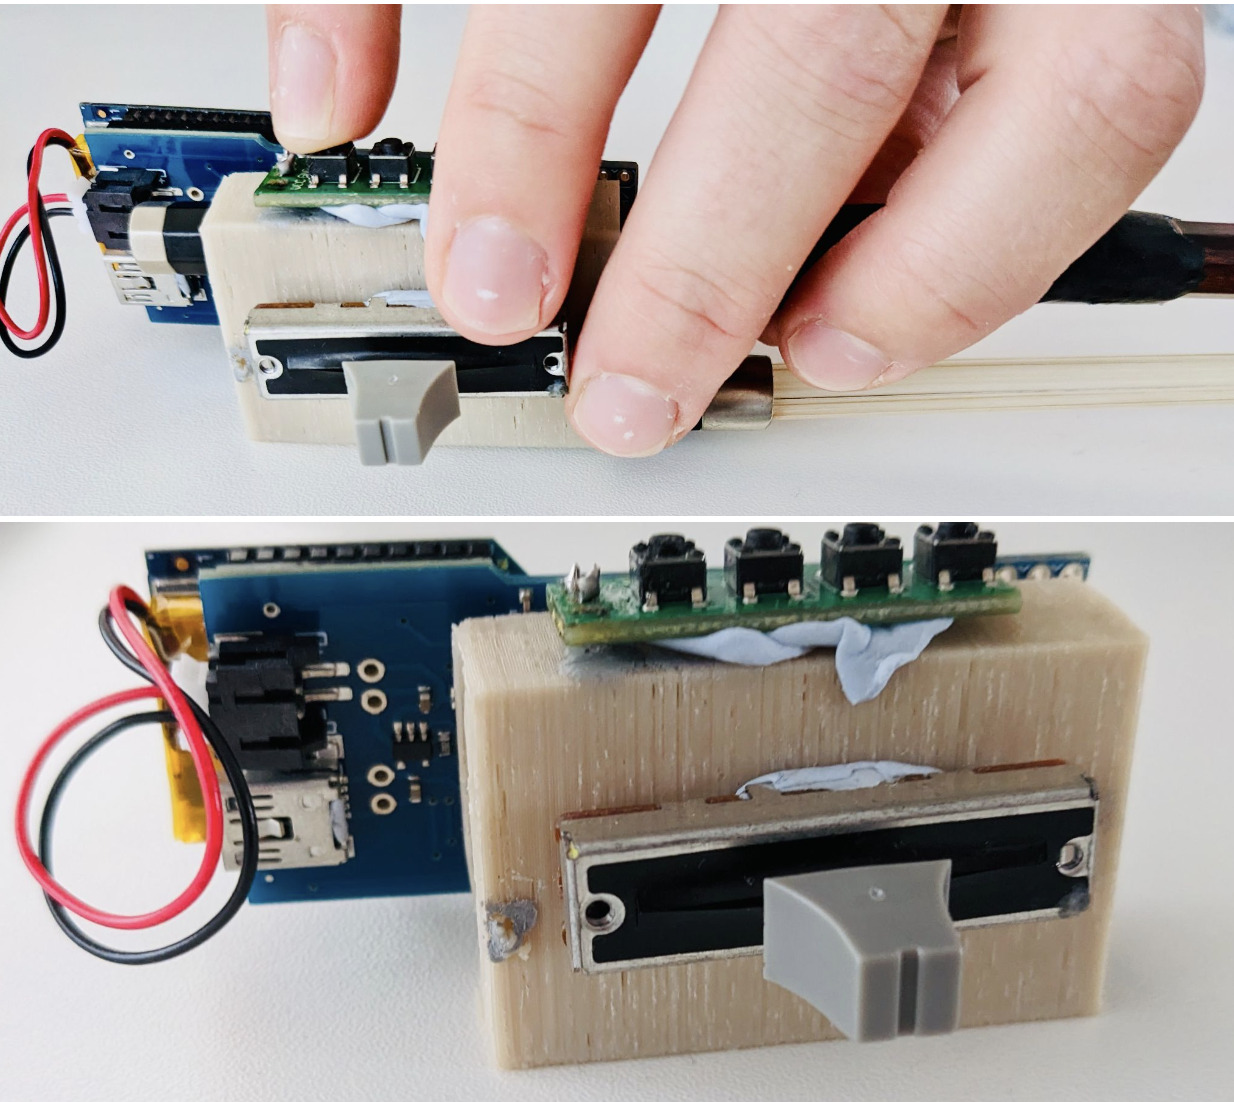
\includegraphics[width=\columnwidth]{newPrototype}
	\caption{Wireless Audio-Visual Violin Bow Interface}
	\label{fig:newPrototype}
\end{figure}

%%not sure what to write here

\newpage
\section{RELATED WORK}

Miranda and Wanderley categorise different types of musical interfaces, with augmented, hyper or hybrid instruments being those that extend the possibilities of an acoustic instrument through the addition of multiple sensors, whilst retaining the instruments original sound and performance gestures\cite{miranda:new}. Significant developments include Diana Young's \textit{Hyperbow Controller}\cite{young:hyperbow}\cite{young:classification},
Machover and Chung's \textit{Hypercello}\cite{levenson:taming}\cite{paradiso:musical}, \textit{vBow} developed by Nichols\cite{nichols:vbow} and Bevilaqua's \textit{Augmented Violin}\cite{bevilacqua:augmented}.With the sensors integrated directly into the acoustic instrument, these new interfaces are designed for detailed analysis of intricate real-time playing gestures\cite{bevilacqua:augmented}, augmenting the possibilities of the instrument, whilst preserving the performer's natural relationship with the instrument.


Building on these concepts but with the design consideration of minimal invasion to the acoustic instrument are Kimura's \textit{Augmented Violin Glove}\cite{kimura:extracting} and Reid's \textit{MIGSI}\cite{Reid:2016} which hold the sensor technology inside a custom designed housing that is made to be both easily integrated and removed. Bevilacqua discusses another approach to augmenting an acoustic instrument which incorporates interactive sensors such as FSRs, push buttons and sliders\cite{bevilacqua:augmented}. 


Although both approaches aim at enhancing and expanding the possibility of an acoustic instrument\cite{machover:interactive}, the latter adds new gestures for the performer\cite{bevilacqua:augmented}\cite{overholt:advancements}.
Ko and Oehlberg's \textit{TRAVIS II}\cite{ko:touch}, allows the performer to trigger a selection of audio and visual presets via four FSRs. The interface technology, designed to augment the fingerboard of the violin,  with the exception of the custom made sensing fingerboard itself, by using 3D printed clamps allows for complete removal of all other sensor technology from the body of the violin . Overholt's \textit{The Overtone Fiddle}\cite{overholt:overtone} combines the retention of traditional technique as well as introducing new extended performance gestures. Though the Overtone Fiddle allows performer control through traditional violin technique, it is an entirely new custom designed instrument with extensive augmentation capabilities.
%both approaches have same results
Despite the variations in physical design considerations, these interfaces all communicate sensor data to appropriate musical software environments which is then used to transform
the traditional acoustic capabilities of the instrument into new musical outcomes\cite{machover:hyperinstrument}. These two design components are therefore of equal significance within the development of a new musical interface.
% It is therefore the software mappings that truly differentiate each interface. 
In the case of concurrent dynamic audio and visual software mappings, various approaches have been explored, including Ali Momeni and Cyrille Henry's introduction of a \textit{Dynamic Independent Visual Mapping Layer}\cite{momeni:dynamic}, Jaroslaw Kapuscinski's \textit{Intermedia}\cite{savery:intermedia}\cite{kapuscinski:7mudras} Bert Bongers and Yolande Harris' \textit{Video-Organ}\cite{bongers:structured} as well as the more recent \textit{AirSticks}\cite{ilsar:airsticks} by Alon Ilsar with real-time interactive visuals designed by Andrew Bluff, Matthew Hughes and others. Our work-in-progress ambitiously aims at incorporating elements from all of these design approaches into one small yet robust musical interface.


\section{Design Motivation}

Coming from a background in classical and jazz violin as well as composition and music technology, the first author spent a considerable amount of time experimenting with various hardware technologies and software environments. These included electric instruments, multi effects pedals and various pickups. Throughout their academic and professional performing arts career, the first author shifted towards an intermedia creative practice, which combined visuals and audio and branching away from commercially available hardware augmentations. The desire to create an audio-visual, wireless interface that would fit on the frog of the violin bow came from wanting to move away from the visual aesthetic of long cables, bulky pedal rigs and other visually and physically restrictive technologies. 



The goal was to create a custom built controller with real-time audio and visual processing capabilities that could be manipulated with just the right hand fingers of an expert violinist, creating a minimally invasive, cost effective, mobile version which effectively combined already existing technologies. 

This design would also allow for easier interdisciplinary collaborations, where the violinist could effortlessly move around the stage and interact with dancers, actors or any digital set component such as a projection surface or lighting design. As a small and mobile device, the interface would retain a sense of mystery and magic within a live performance, where the audience would not be distracted by the interface and the process of audio and visual manipulation. An aesthetic that is otherwise very present when using an electric instrument or a foot pedal. As a custom built controller, the interface would be designed around the physical and technical capabilities of the violinist, with optimal sensor placement and a software mapping system. 

% - 

% - my Capstone recital incorporated a four movement work for mixed ensemble, interactive visuals, a dancer and electronics \cite{savery:intermedia}. The four movements were connected by a recurring theme of a heartbeat. 

%  My vision for the interactive visuals was to be exclusively derived from live audio analysis, using Sigmund~. However, the results were not consistent, and in order to save time, a Keith McMillan SoftStep was used, despite the time it took to physically incorporate foot triggering into each piece. 
%  Similarly to Mari Kimura  \cite{kimura:creative}, the physical action of pushing an effects pedal with my foot, whilst playing and having to remain in one place felt unnatural and distracting. I also wanted to maintain a sense of magic and mystery for the audience, a sentiment shared by Kimura \cite{kimura:creative} and Jensenius and Johnson \cite{Jensenius:performing}. Ilsar also stresses the importance of magic in electro-acoustic music and compositions, as a source of disembodied sound \cite{ilsar:airsticks}. Unlike an acoustic instrument, which is a direct source of sound, electro-acoustic and electronic sounds create a disconnect from its source, creating an atmosphere of mystery and illusion. A concept diffused by the choreographed act of triggering changes in sound processing by suppressing a foot pedal.
%  A wireless, discretely designed controller with sophisticated software mappings creates a subtle and discrete presence.
 
%  It would also allow the performer more freedom of movement during a live performance, especially when coupled with a wireless microphone.
 
%  One approach to solving the issue of freedom of movement is explored by by Jensenius and Johnson \cite{Jensenius:performing} using a video-based motion-tracking system with a suspended camera above the stage which together allow the performer to move freely on stage whilst retaining full control over the electronics \cite{Jensenius:performing}. 
%  % talk about violinist
%  Jensenius and Johnson state that the setup allows the violinist to improvise with the electronic sounds whilst moving around what they describe as a sonic space \cite{Jensenius:performing}. The goal of the project was to create an invisible technological setup that still allowed for great control of live electronics as well as allowing for musically interesting interactions between the performer and electronics. I wanted to achieve a similar degree of freedom and control with a minimally invasive, removable interface, and without having to rely on external devices such as suspended cameras or motion tracking systems. 

\section{Implementation}

We began to design the physical interface by testing a variety of different sensors with the Arduino and Max/MSP software. Short snippets of live violin audio were recorded and then manipulated by the sensors which were either attached to a breadboard or simply laid out on a desk. This physical and software prototyping process lasted about three months, involving a cyclical practice based research approach of practice, theory and evaluation\cite{candy:practice}\cite{candy:guide}, where an idea for an audio-visual work would be realised and tested, accumulating in a series of Max abstractions and an Arduino sketch that could then be used in a larger, more cohesive composition. As the music became predominantly loop based, we decided to shift to Max for Live, and control its parameters via the live object model\footnote{\url{https://docs.cycling74.com/max8/vignettes/live_object_model}}.

%add picture here

\subsection{Physical Design}


%expand on this in the virtual section

The goal of creating this interface was to make a real-time controller capable of audio and visual processing through direct manipulation of right hand fingers. As a starting point of the design process, we began working with just two controller sensors. These were a potentiometer slider\footnote{
Adafruit Slider Trinkey - USB NeoPixel Slide Potentiometer}, and a four button keypad\footnote{Vanki Arduino keypad 4 Button Key Module Switch Keyboard for UNO MEGA2560}. These were chosen for ease of both physical interaction and initial software mappings. 
In order to facilitate the wireless design consideration, we chose to work with the XBee ZB Zigbee wireless modules\footnote{\url{https://www.digi.com/resources/examples-guides/basic-xbee-zb-zigbee-(series-2)-chat}}, mounting the radio module directly onto an Arduino Fio board. 

Another design consideration was making sure the interface was easily removable from the frog of the bow. This was important as the interface is intended for use by an expert practitioner and their professional instrument setup. This was enabled through the design of a series of 3D printed casings, that slid on and off the bow. Multiple iterations were needed, as the rigidity of the casings did not allow for slight variations in bow frog dimensions. The sensors were then mounted onto the chosen casing using various adhesives. As an initial physical prototyping model, this approach worked well, allowing for rapidly exploring different sensor placement positions in order to find an optimal one. However, in a live performance setting, these adhesives were not secure enough and both the casing and the sensors shifted around too much. 

%add photo here.

\begin{figure}[t]
	\centering
		\includegraphics[width=0.5\columnwidth]{3d casings}
	\caption{Examples of 3D printed casings}
	\label{fig:3d casings}
\end{figure}
 % The constraint of having all the sensors being located on the interface meant having to make early decisions about its physical design. My co-supervisor, Dr Sam Ferguson suggested that an XBee radio module would be the most discrete and reliable platform for sending wireless data, as it eliminates relying on WiFi and Bluetooth, having had successful experiences with the unit in such projects as fellow Creativity and Cognition Studio PhD graduate, Alex Murray-Leslie, where the electronics were embedded within a custom-built E-Shoe  \cite{murray:liberation}. The XBee radio unit, mounted onto an Arduino Fio board and an Xbee USB explorer on the receiving end have also been used by new musical interface developers, Sarah Bell Reid  \cite{Reid:2016} within her Minimally Invasive Gesture Sensing Interface (MIGSI) for trumpet and Johnson Et al. with their \textit{MusikJacket} - an educational tool that provides real-time feedback to assist beginner violinists in learning the instrument with appropriate posture \cite{van:musicjacket}. 






\subsection{Software Design}

After successful data communication between the sensors, Arduino and Max software was established, we focused on deciding how to best approach software mappings in order to achieve robust and creatively meaningful results. We decided to approach this problem using a practice led trajectory, where a live audio-visual work for solo violin and the interface was used as a means to develop a series of criteria for software mappings and compositional approaches\cite{candy:practice}. 

\begin{figure}[t]
	\centering
		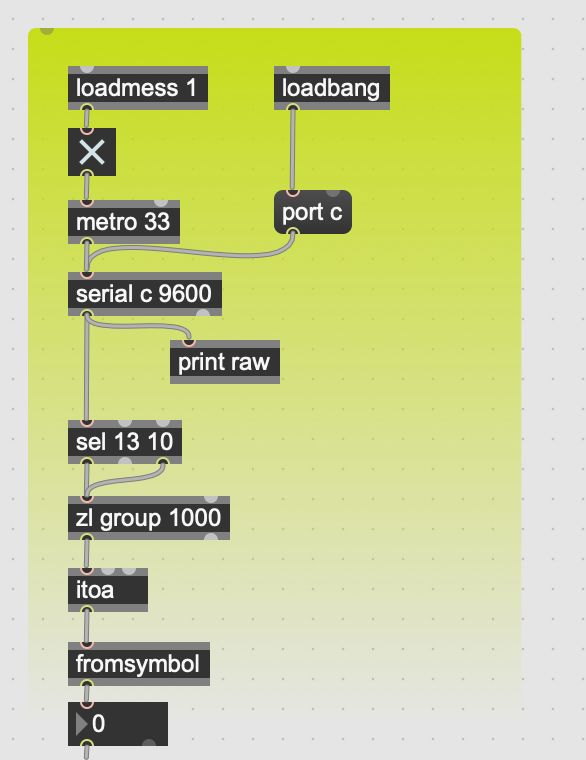
\includegraphics[width=0.5\columnwidth]{serial_max}
	\caption{An abstraction for receiving sensor data from Arduino software}
	\label{fig:serial_max}
\end{figure}

\subsubsection{Audio Mapping}
The four buttons functioned as toggles, with the data mapped to trigger on and off signals. This data was used to control various parameters in Ableton using the live.object and live.path objects. These included triggering clip recordings, looping on and off and deleting recorded clips in real-time. The potentiometer slider data was scaled in a variety of ways, depending on the current section of the composition. 

At times, the data was scaled to receive floats between 0. and 100., where the range of those numbers would control sliders of in-built Max for Live objects, such as the Dry/Wet signals of the Insinkorator or Dual Harmonizer. In other instances, the slider data would be scaled to a range between 0 and 3, acting as a secondary series of buttons, with each integer linked to a direct parameter, such as opening and closing of a gate object or starting and stopping playback of a buffer. 

\begin{figure}[t]
	\centering
		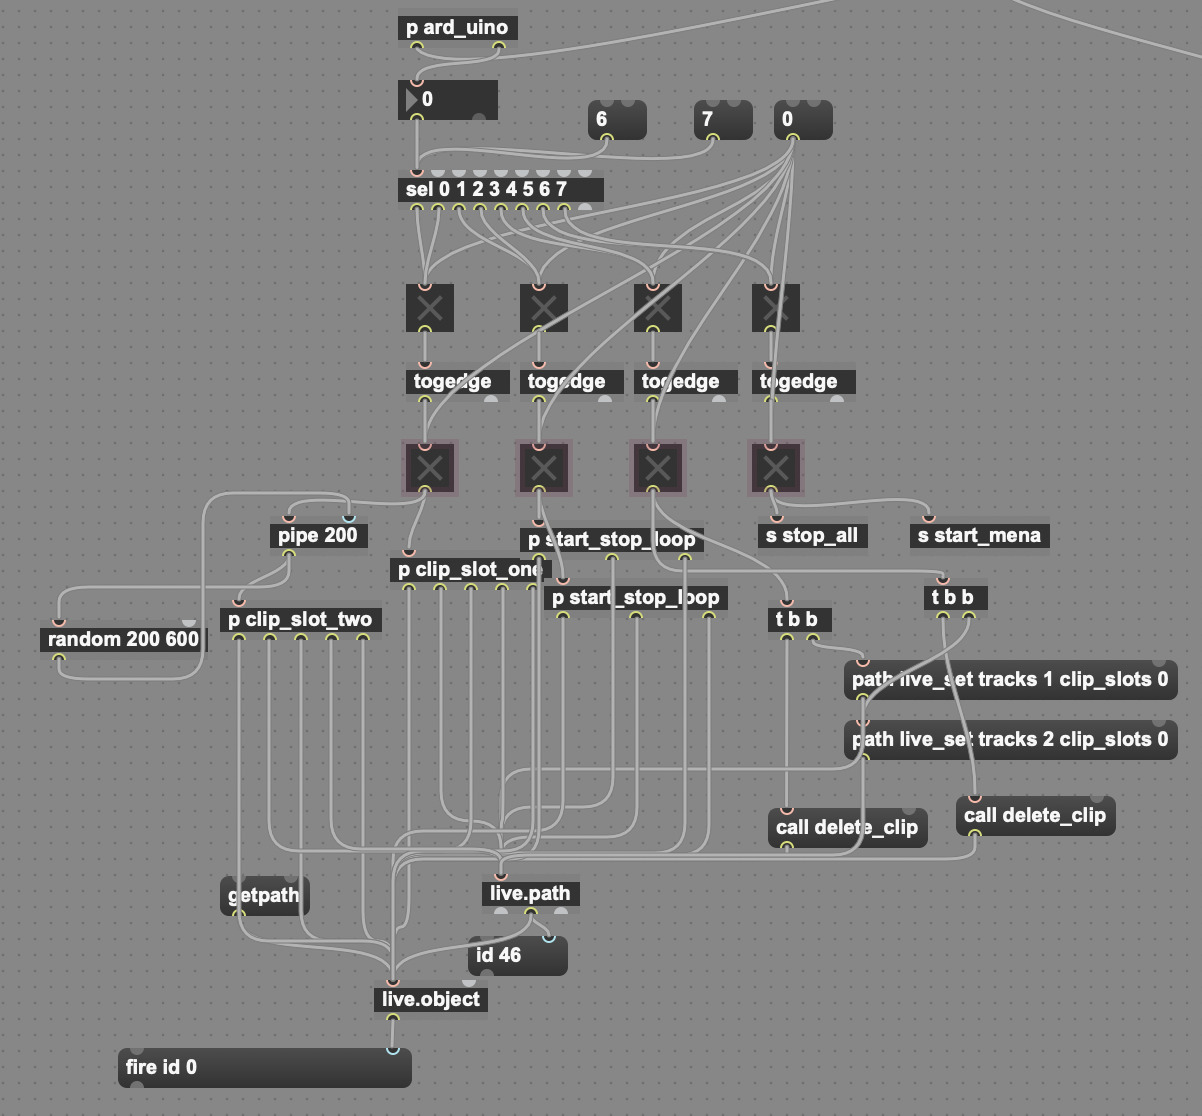
\includegraphics[width=1\columnwidth]{audio}
	\caption{Max for Live patch with audio mappings}
	\label{fig:audio}
\end{figure}

\subsubsection{Visual Mapping}
All visual elements for this initial prototype were processed in Jitter and consisted of video footage. A variety of processing techniques were explored, such as cross-fading between multiple video streams and brightness and controlling contrast and saturation using the jit.brcosa object. These techniques were well suited to being controlled by the potentiometer slider with its analog data stream being easily scaled to range from 0. to 1. 

The biggest mapping challenge was switching or moving between parameters, much like any transition within a piece. Attempting to control multiple parameters simultaneously proved to be somewhat chaotic and less meaningful. One solution was to outline distinct sections within each piece, marked by a counter object in Max. At specific moments throughout a piece, the counter would trigger an opening or closing of a gate object, that would transition from current section to the next. This approach eased the load off the two existing sensors and allowed for more elaborate mappings within each section. However, this also created a very rigid structure, leaving little room for spontaneity.

\begin{figure}[t]
	\centering
		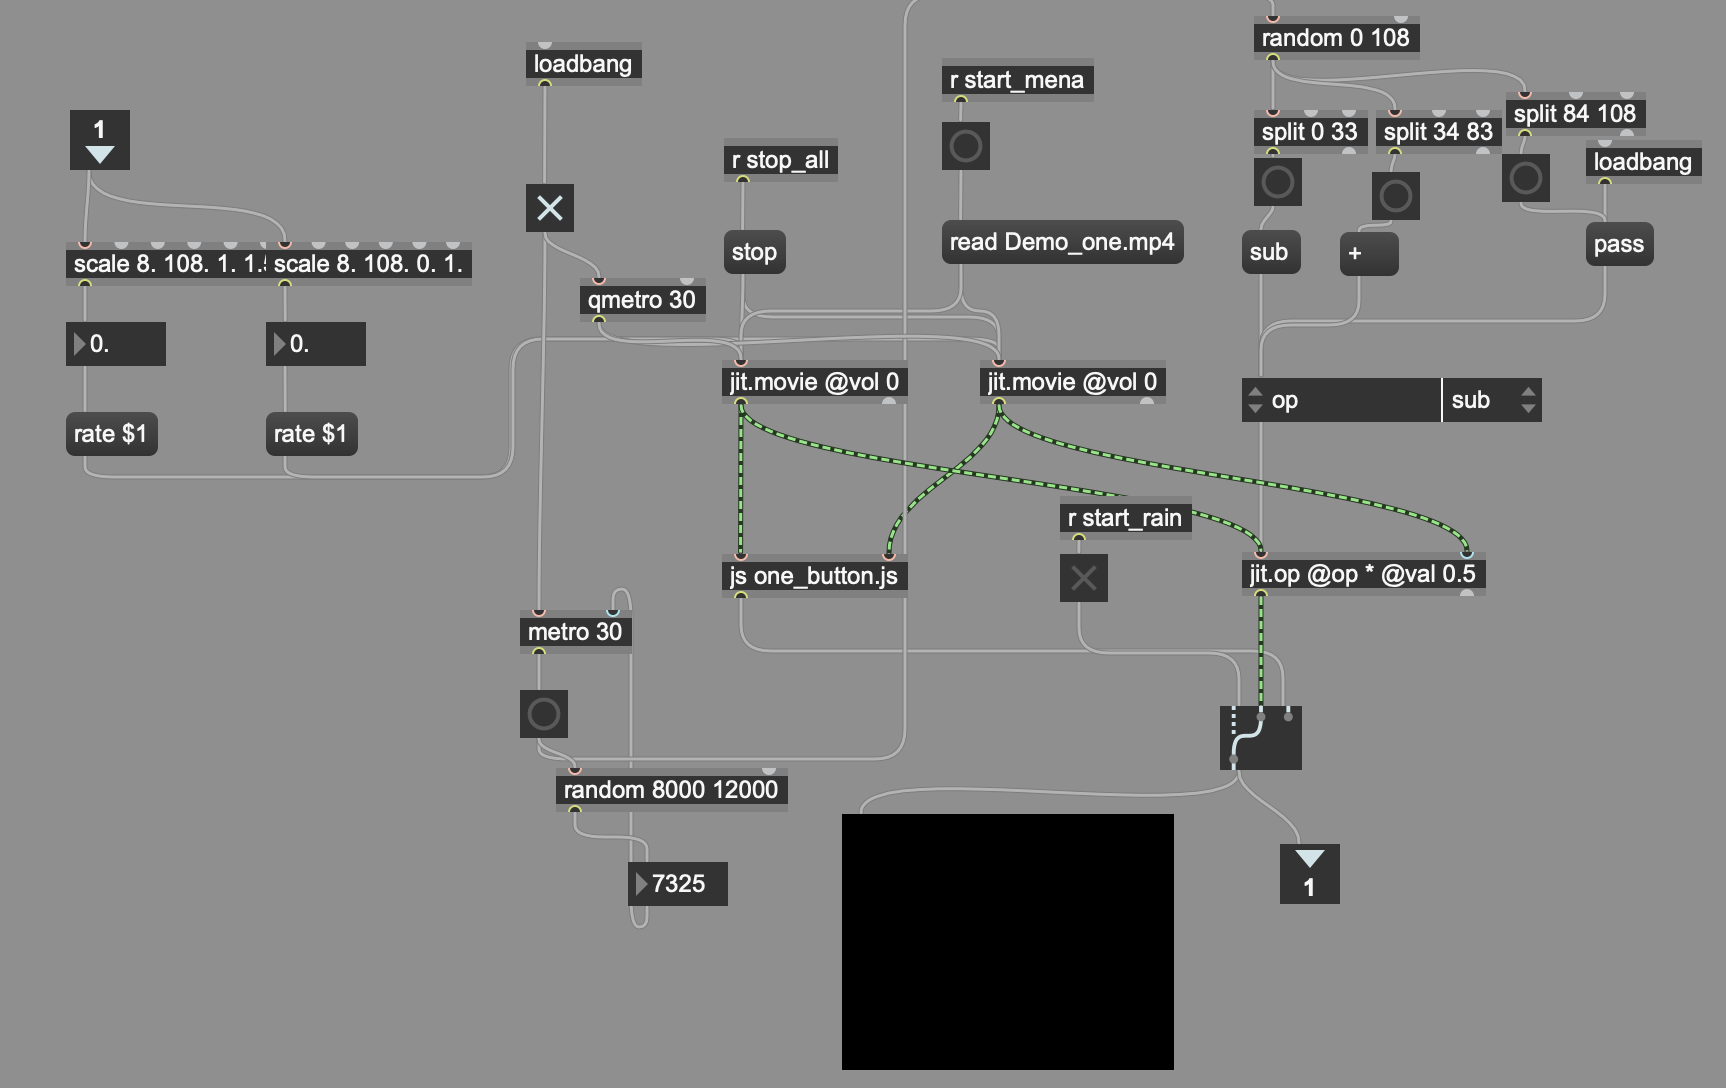
\includegraphics[width=1\columnwidth]{video}
	\caption{Max for Live patch with video mappings using Jitter}
	\label{fig:video}
\end{figure}

\section{Creative Outputs}
We developed and performed  two works using the initial working prototype. The first performance situation the interface was used for was a demonstration video that was filmed in June of 2022. The piece was a combination of a free solo violin improvisation as well as some predetermined structural constraints and a prerecorded audio sample played on viola, which ultimately dictated the harmonic structure and mood of the work. The second performance  situation was a cross university collaboration between University of Technology Sydney and Macquarie University. A robotic arm was used to visualise the first author's playing in real-time using paint on canvas. This performance situation took place over one day with multiple iterations of the piece and visualisations.


\subsection{Demonstration Recording}

In June of 2022A, we filmed a live recording of a demonstration video at the University of Technology Sydney . The composition for solo violin and interface was approximately four minutes in length, and consisted of prerecorded viola samples, live audio sampling and processing and live video processing. The composition was a culmination of the theoretical frameworks developed throughout the period of January 2022 up to June of that year. Musically, the composition was a combination of an improvisation and structured sections, dictated by a Max for Live patch. There were loosely three sections;

A free improvisation with live audio sampling and processing using the Instinkorator audio effect. The recording, playback and looping all triggered by push buttons on the interface. The video footage was initiated with the same push button used to process audio. Brightness and cross fading was controlled by the potentiometer slider.

The second section was triggered by a different push button, which triggered the playback of a prerecorded viola melody. Real-time improvised violin melodies were layered on top of this sample, with further layers created by short real-time sample playback. Each sample being between 10 and 30 seconds in length, with various effects, such as reverse playback, changed playback rate and various harmonizers. For the video footage, this section switched to saturation, but cross fading remained. 

The last section deleted the short audio samples one by one, thinning out the layers and creating a natural decrease in volume, descending into an ending. The video footage played out to the end and came to a natural pause as the patch stopped. 

Link to video
\href{https://www.dropbox.com/s/yk6e073fcjxtjfu/NIME_demo.mp4?dl=0}{here} 

% \footnote{Link to demonstration video recording\url{https://youtu.be/Z66rgnPBrXI}}

\begin{figure}[t]
	\centering
		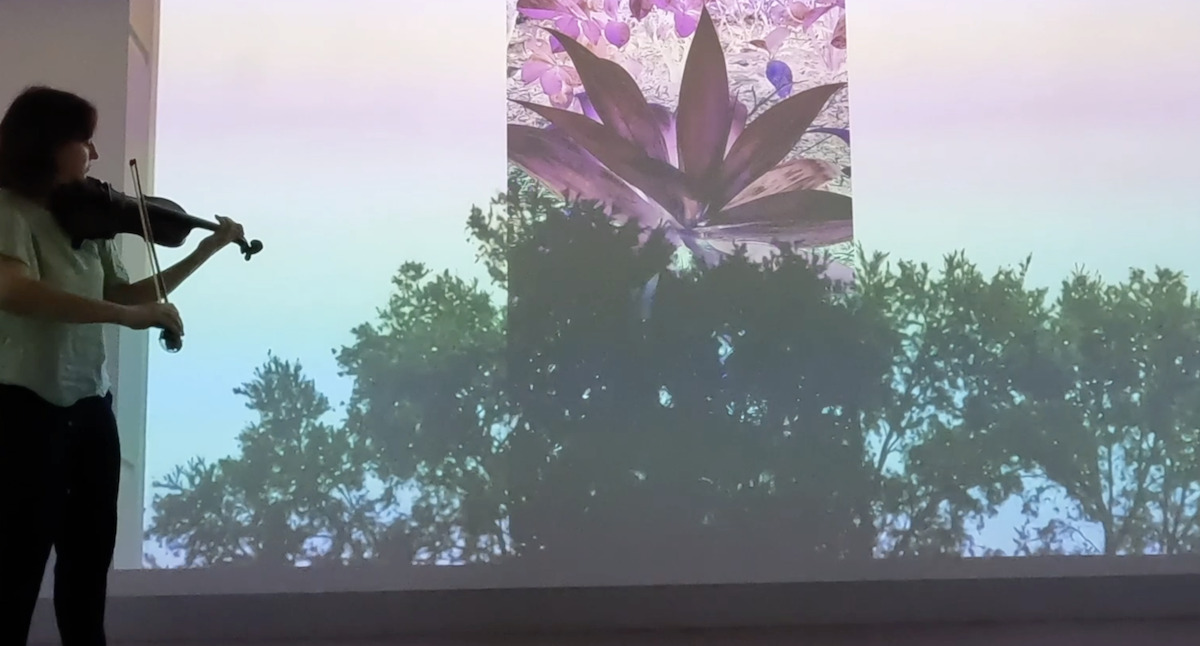
\includegraphics[width=0.6\columnwidth]{Performance1}
	\caption{Demonstration video recording}
	\label{fig:Performance1}
\end{figure}

\subsection{Reflection}

With most of the design focus being centered on the physical implementation and software mappings, the musical development was unfortunately a secondary priority. This became very evident when the piece became predominantly a free improvisation, with harmonic and rhythmic elements consisting solely of the prerecorded viola sample. Manipulating the sensors with right hand fingers whilst playing also proved to be surprisingly challenging, partially due to the physical design of the interface, where the sensors were not optimally placed for efficient manipulation, but also due to the mental load of performing and incorporating new gestures into that performance required to manipulate the interface sensors. 

\subsection{Performance Visualisation}

Similar to the demonstration video, this was mostly a free improvisation, with a structure revolving around a time constraint of approximately 8 minutes. This is approximately how long it took the robotic arm to fill the canvas using all four available paint colours. Audio effects were worked out to align with paint color changes and the corresponding layering and mixing of paint on canvas. Hence, the piece always began with solo violin and black paint. 

When the robotic arm was ready to add a blue color to the canvas, a push button on the audio-visual interface was used to trigger an addition of the Max for Live dual harmonizer audio effect. The potentiometer slider was used alternate between two octaves below and two octaves above the real-time audio from the violin. This thickened out the sonic texture, aligning with the painted canvas. 

From the onset of the piece, short live audio samples of approximately 10-20 seconds in length were being recorded. Each with a separate audio effect. Using a push button again, the dual harmonizer was gated off and the recorded audio samples would start looping one by one, thickening out the sonic texture more and more, as the robotic arm added yellow and then red. The piece finished on a large crescendo as the canvas filled with vibrant colors and a variety of short and long strokes\cite{savery:robotic}.

Link to video \href{https://www.dropbox.com/s/fu38a4jx1ph0x9t/Tesseract%20POC.mp4?dl=0}{here}

\begin{figure}[t]
	\centering
		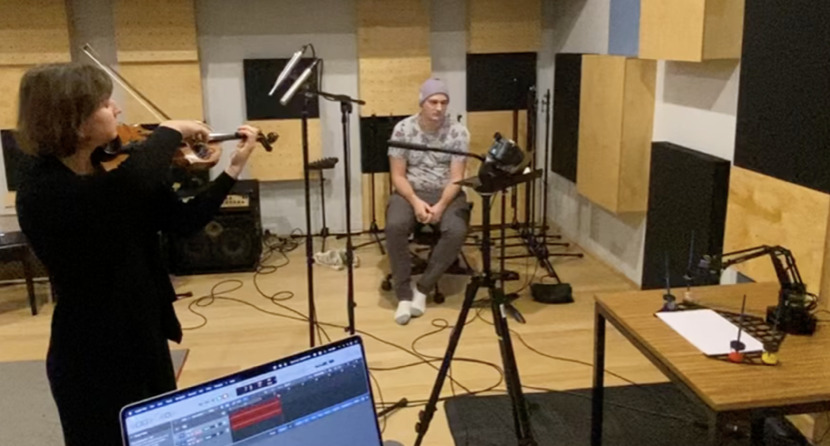
\includegraphics[width=0.5\columnwidth]{performance2}
	\caption{Rehearsing with the robot painting arm}
	\label{fig:performance2}
\end{figure}
\begin{figure}[t]
	\centering
		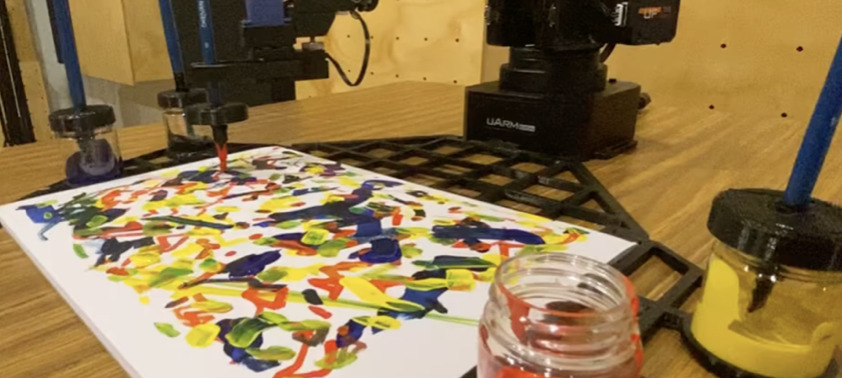
\includegraphics[width=0.5\columnwidth]{canvas}
	\caption{Completed canvas}
	\label{fig:canvas}
\end{figure}

\subsection{Reflection}

The absence of a visual component from the interface in this work allowed for a deeper investment into the audio mappings. Since this collaboration followed the demonstration video recording, many of the physical and virtual parameters were already flushed out and familiar. This allowed the first author to focus more on the musical aspects of the performance whilst becoming accustomed to responding to a robotic arm collaborator. 

The physical manipulation of the interface became somewhat easier after re-evaluating the demonstration video recording and relocating the sensors to different parts of the casing. We moved the push button panel was moved slightly higher up the bow to stop the right hand pinkie from involuntarily suppressing the outer most button during bow changes and lifts. The potentiometer slider was also moved slightly to the left, away from the bow screw to allow for better reach from the right hand middle finger, which is used to manipulate the sensor.

\section{Conclusion and Future Work}
The wireless audio-visual violin bow interface described in this paper has laid a strong foundation for the next iteration of this ongoing research project. This prototype has been a robust proof of concept, showing that a wireless sensor enhanced interface can be successfully manipulated in real-time by a violinist's right hand fingers within a variety live performance situations. The work-in-progress prototype has also successfully demonstrated that both audio and visuals can be concurrently developed and processed, opening up a wide potential for future creative output and interactive audio-visual system design.

A more recent version of the interface is using a silicone encasement for the sensors, which can slide on and off the bow frog. This more flexible material allows for discrepancies in bow size whilst retaining the sensors in place securely during a live performance situation. Two more sensors have been added to this version; a force sensor, that is fitted on the outside of the silicone casing bellow the bow frog for manipulation with the right hand thumb and a 3-axis acceleromter, mounted on the side of the Arduino Fio board. The latter, with representation of nuanced gestures through its data flow, will require a considerable amount of practice and performance experience to fully develop and master. Two Flora neopixel LEDs have also been added for visual feedback so as to avoid external help and create a more trusting relationship between the system and the performer\cite{kimura:creative}.

The design focus for future works is predominantly preoccupied with software mappings. The initial steps are aimed at developing a modular approach to both audio and visual mappings for each sensor, similar to approaches taken by Bonger and Harris in the development of the 
\textit{Video-Organ}\cite{bongers:structured}. This will allow for spontaneity in live performance situations, easier collaborations with other artists and propel robust composition ideas. After this design process, we will focus on developing a more autonomous software system, where the audio and visual elements will have some component of agency and interaction, resembling the directions taken by some of the works incorporating 
Ilsar's \textit{AirSticks} 
such as \textit{H2.O}
\cite{ilsar:airsticks}. 






\section{Acknowledgments}


This research is supported by an Australian Government Research Training Program Scholarship.



\bibliographystyle{abbrv}
\bibliography{nime-references} 

\end{document}
